\chapter{Aspectos teóricos y revisión de la literatura}
\section{Aspectos teóricos}
\subsection{Algoritmo de retropropagación}
Una regla de aprendizaje es el método que le permite adaptar los parámetros de la red. El perceptrón multicapa actualiza sus pesos en función de la salida obtenida de tal manera que los nuevos pesos permitan reducir el error de salida. Por tanto, para cada patrón de entrada a la red es necesario disponer de un patrón de salida deseada.

El objetivo es que la salida de la red sea lo más próxima posible a la salida deseada, debido a esto la es que el aprendizaje de la red se describe como un problema de minimización de la siguiente maner $$ \min_{W} E $$ donde $W$ es el conjunto de parámetros de la red (pesos y umbrales) y $E$ es una función de error que evalúa la diferencia entre las salidas de la red y las salidas deseadas. en la mayor parte de los casos, la función de error se define como:
\begin{eqnarray}
	E = \frac{1}{N}\sum^{N}_{i = 1} e(i)
\end{eqnarray}

Donde $N$ es el número de muestras y $e(n)$ es el error cometido por la red para el patrón $i$, definido de la siguiente manera
\begin{eqnarray}
	e(i) = \frac{1}{n_{C}}\sum^{n_{C}}_{j = 1} (s_{j}(i) - y^{j}(n))^2\label{eq:error_patron}
\end{eqnarray}

Siendo $Y(i) = (y_{1}(i), y_{2}(i), \cdots, y_{n_{C}}(i))$ y $S(i) = (s_{1}(i), s_{2}(i), \cdots, s_{n_{C}}(i))$ los vectores de salida y salidas deseadas para el patrón $i$ respectivamente.

De esta manera, si $W^{*}$ es un mínimo de la función de error $E$, en dicho punto el error será cercano a cero, y en consecuencia, la salida de la red será próxima a la salida deseada.

Así es como el aprendizaje es equivalente a encontrar un mínimo de la función de error. La presencia de funciones de activación no lineales hace que la respuesta de la red sea no lineal respecto a los parámetros ajustables, por lo que el problema de aminimización es un problema no lineal y se hace necesario el uso de técnicas de optización no lineales para su resolución.

Las técnicas utilizadas suelen basarse en la actualización de los parámetros de la red mediante la determinación de una dirección de búsqueda. En el caso de las redes neuronales multicapa, la dirección de búsqueda más utilizada se basa en la dirección contraria del gradiente de la función de error $E$, el método de gradiente descendente.

Si bien el aprendizaje de la red busca minimizar el error total de la red, el procedimiento está basado en métodos del agradiente estocástico, que son una sucesión de minimizaciones del error en función de cada patrón $e(i)$, en lugar de minimizar el error total $E$ de la red. Aplicando el método del gradiente estocástico, cada parámetro $w$ se modifica para cada patrón de entrada $n$ según la siguiente regla de aprendizaje
\begin{eqnarray}
	w(i) = w(n - 1) - \alpha\frac{\partial e(i)}{\partial w}
\end{eqnarray}

donde $e(i)$ es el error para el patrón de entrada $i$ dado por la ecuación \ref{eq:error_patron}, y $\alpha$ es la tasa de aprendizaje, éste último determina el desplazamiento en la superficie del error.

Como las neuronas están ordenadas por capas y en distintos niveles, es posible aplicar el método del gradiente de forma eficiente, resultando en el {\em algoritmo de retropropagación} \cite{Rumelhart1986} o {\em regla delta generalizada}. El término retropropagación es utilizado debido a la forma de implementar el método del gradiente en las redes multicapa, pues el error cometido en la salida de la red es propagado hacia atrás, transformándolo en un error para cada una de las neuronas ocultas de la red.

% Neural Networks for Pattern Recognition - Bishop: 140 - Error backpropagation.
% Neural Networks for Pattern Recognition - Bishop: 263 - Gradient descent.
El algoritmo de retropropagación es el método de entrenamiento más utilizado en redes con conexión hacia adelante. Es un método de aprendizaje supervisado de gradiente descendente, en el que se distinguen claramente dos fases:
\begin{enumerate}
	\item Se aplica un patrón de entrada, el cual se propaga por las distintas capas que componen la red hasta producir la salida de la misma. Esta salida se compara con la salida deseada y se calcula el error cometido por cada neurona de salida.

	\item Estos errores se transmiten desde la capa de salida, hacia todas neuronas de las capas anteriores \cite{Fritsch1996}. Cada neurona recibe un error que es proporcional a su contribución sobre el error total de la red. Basándose en el error recibido, se ajustan los errores de los pesos sinápticos de cada neurona.
\end{enumerate}

\subsection{Problema desl desvanecimiento del gradiente}
El problema del gradiente desvaneciente nace en las NN profundas, éstas utilizan funciones cuyo gradiente tienden a estar entre 0 y 1. Debido a que estos gradientes pequeños se multiplican durante la retropropagación, tienden a {\em desvanecerse} a través de las capas, evitando que la red aprenda en redes muy profundas.

%%%% VER QUE LA NOTACIÓN SEA COMPATIBLE
Si se tiene una NN, la activación de una neurona de una capa intermedia $i$ con función de activación $f_i$ y con entrada $$ net_{i}(t) = \sum_{j}w_{ij}y^{j}(t - 1) $$ es $y^{i}(t) = f_{i}(net_{i}(t))$. Además $w_{ij}$ es el peso de la conexión desde la unidad $j$ hasta la unidad $i$, $d_{k}(t)$ será la respuesta esperada de la unidad $k$ de la capa de salida en el tiempo $t$. Usando el error cuadrático medio ({\em Mean square error}, MSE), el error de $k$ será
$$ E_{k}(t) = (d_{k}(t) - y^{k}(t))^2 $$

En un tiempo $\tau \leq t$ cualquiera, el error de una neurona $j$ que no sea una neurona de entrada es la suma de los errores externos y el error propagado hacia atrás desde la neurona previa será
$$ \vartheta_{j}(\tau) = f'_{j}(net_{j}(\tau))\left(E_{j}(\tau) + \sum_{i} w_{ij}\vartheta_{i}(\tau + 1)\right) $$

El peso actualizado en el tiempo $\tau$ resulta
$$ w_{jl}^{new} = w_{jl}^{old} + \alpha\vartheta_{j}(\tau) y^{l}(\tau - 1)$$
donde $\alpha$ es la tasa de aprendizaje, y $l$ es una unidad arbitraria conectada a la unidad $j$.

En un tiempo arbitrario $\tau \leq t$, el error de la señal en una unidad $j$, que no sea de entrada, será la suma de los errores externos y la señal propagada anterioremente como muestra la ecuación \ref{eq:propagation_error}.
\begin{eqnarray}
	\vartheta(\tau) &=& f'_{j}(net_{j}(\tau)) \left(E_{j}(\tau) + \sum_{i}w_{ij}\vartheta_{i}(\tau + 1)\right)
	\label{eq:propagation_error}
\end{eqnarray}

Entonces, los pesos actualizados serán $$ w_{jl}^{new} = w_{jl}^{old} + \alpha\vartheta_{j}(\tau)y^{l}(\tau - 1) $$
\begin{comment}
Error en el factor de escala. Véase también las contribuciones anteriroes al análisis del desvanecimiento del gradiente \cite{Hochreiter1997a, Bengio1994, Hochreiter1991}. Propagando el error de una unidad $u$ en el timpo $t$ hacia una unidad $v$ {\Huge for $q$ time steps}, el error escala como muestra la ecuación \ref{eq:scale_error}
\begin{eqnarray}
	\frac{\partial \vartheta_{v}(t - q)}{\partial \vartheta_{u}(t)}
	&=&
	\left\{
	\begin{array}{lr}
		f'_{v}(net_{v}(t - 1))w_{uv}&q=1\\
		\\
		f'_{v}(net_{v}(t - q))\sum^{n}_{l = 1}\frac{\partial \vartheta_{l}(t - q + 1)}{\partial \vartheta_{u}(t)}w_{lv}	&q > 1
	\end{array}
	\right.\label{eq:scale_error}
\end{eqnarray}
\end{comment}

\begin{imagen}
	\scalebox{1.0}{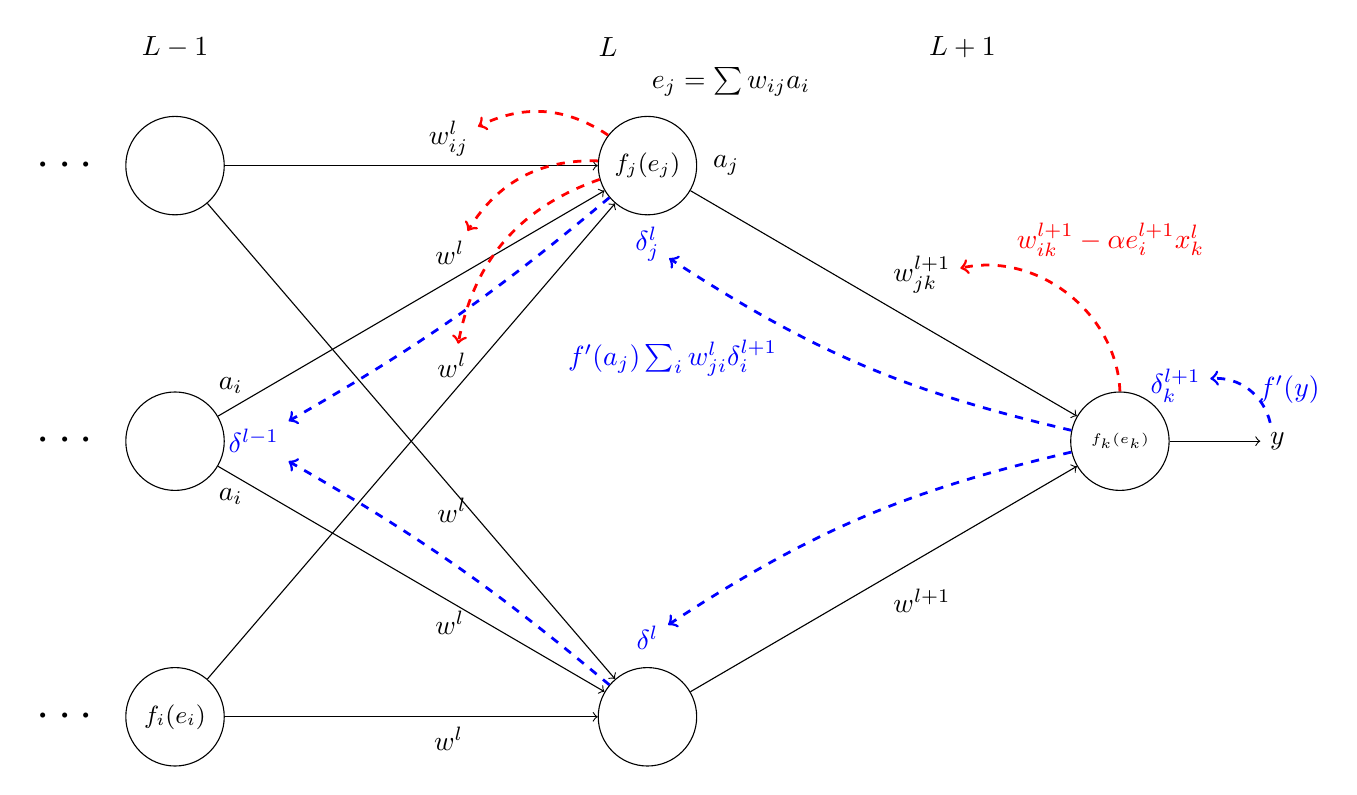
\begin{tikzpicture}

	\tikzstyle{nodo}=[circle, draw, minimum size=1.25cm]
	\tikzstyle{upw}=[dashed, red, ->, line width = 1pt]

	\coordinate (l_0) at (0, 5.0);
	\coordinate (l_1) at (5.5, 5.0);
	\coordinate (l_2) at (10, 5.0);

	\coordinate (f_1_1) at (0, 3.5); % CAPA ENTRADA
	\coordinate (f_1_2) at (0, 0); % CAPA ENTRADA
	\coordinate (f_1_3) at (0, -3.5); % CAPA ENTRADA
	\coordinate (f_2_1) at (6.0, 3.5); % CAPA OCULTA 1
	\coordinate (f_2_2) at (6.0, -3.5); % CAPA OCULTA 1
	\coordinate (f_3_1) at (12, 0); % CAPA SALIDA
	\coordinate (y) at (14, 0); % CAPA SALIDA

	\node[] (l_0) at (l_0) {$L - 1$};
	\node[] (l_1) at (l_1) {$L$};
	\node[] (l_2) at (l_2) {$L + 1$};

	\node[nodo] (f_1_1) at (f_1_1) {}; % CAPA ENTRADA
	\node[nodo] (f_1_2) at (f_1_2) {}; % CAPA ENTRADA
	\node[nodo] (f_1_3) at (f_1_3) {\small $f_i(e_i)$}; % CAPA ENTRADA
	\node[nodo] (f_2_1) at (f_2_1) {\small $f_j(e_j)$}; % CAPA OCULTA 1
	\node[nodo] (f_2_2) at (f_2_2) {}; % CAPA OCULTA 1
	\node[nodo] (f_3_1) at (f_3_1) {\tiny $f_k(e_k)$}; % CAPA SALIDA
	\node[] (y) at (y) {$y$}; % CAPA SALIDA

	\node[left of=f_1_1, node distance=1.4cm] {\LARGE $\cdots$};
	\node[left of=f_1_2, node distance=1.4cm] {\LARGE $\cdots$};
	\node[left of=f_1_3, node distance=1.4cm] {\LARGE $\cdots$};

	\draw[->] (f_1_1) -- node[pos=0.6, above] (w_1_1) {$w^{l}_{ij}$} (f_2_1);
	\draw[->] (f_1_2) -- node[pos=0.6, above] (w_1_2) {$w^{l}_{}$} (f_2_1);
	\draw[->] (f_1_3) -- node[pos=0.6, above] (w_1_3) {$w^{l}_{}$} (f_2_1);
	\draw[->] (f_1_1) node[above right of=f_1_2] {$a_{i}$} -- node[pos=0.6, below] (w_2_1) {$w^{l}_{}$} (f_2_2);
	\draw[->] (f_1_2) node[below right of=f_1_2] {$a_{i}$} -- node[pos=0.6, below] (w_2_2) {$w^{l}_{}$} (f_2_2);
	\draw[->] (f_1_3) -- node[pos=0.6, below] (w_2_3) {$w^{l}_{}$} (f_2_2);
	\draw[->] (f_2_1) node[right of=f_2_1] {$a_{j}$} -- node[pos=0.5, above right] (w_j_k) {$w^{l+1}_{jk}$} (f_3_1);
	\draw[->] (f_2_2) -- node[pos=0.5, below right] {$w^{l+1}$} (f_3_1);
	\draw[->] (f_3_1) -- node[pos=0.5, below right] {$$} (y);

	\node[above right of=f_2_1, node distance=1.5cm] {$e_{j} = \sum w_{ij}a_i$};


	\draw[upw] (f_3_1) to[bend right=50] node[above right, pos=0.8] {$w^{l+1}_{ik} - \alpha e^{l+1}_{i}x^{l}_{k}$} (w_j_k);
	\draw[upw] (f_2_1) to[bend right=30] node[above]{$$} (w_1_1);
	\draw[upw] (f_2_1) to[bend right=30] node[above]{$$} (w_1_2);
	\draw[upw] (f_2_1) to[bend right=30] node[above]{$$} (w_1_3);


	\node[blue, above right of=f_3_1] (e_i) {$\delta^{l+1}_{k}$};
	\node[blue, below of=f_2_1] (e_2_1_i) {$\delta^{l}_{j}$};
	\node[blue, above of=f_2_2] (e_2_2_i) {$\delta^{l}$};
	\node[blue, right of=f_1_2] (e_1_2_i) {$\delta^{l-1}$};

	\draw[upw, blue] (y) to[bend right=40] node[right]{$f'(y)$} (e_i);
	\draw[upw, blue] (f_3_1) to[bend left=10] node[below left, pos=0.7]{$f'(a_{j})\sum_{i}w^{l}_{ji}\delta^{l+1}_{i}$} (e_2_1_i);
	\draw[upw, blue] (f_3_1) to[bend right=10] (e_2_2_i);

	\draw[upw, blue] (f_2_1) to[bend left=5] (e_1_2_i);
	\draw[upw, blue] (f_2_2) to[bend right=5] (e_1_2_i);

\end{tikzpicture}
}
	\label{fig:vanishing}
	\caption{Gradiente descendente}
\end{imagen}

\section{Revisión de la literatura}
